\section{Theorie}
\label{sec:Theorie}

\subsection{LC-Kreis}
\label{sec:lckreis}
Der LC-Kreis enthält eine Spule mit Induktivität $L$ und einen Kondensator mit Kapazität $C$ (siehe Abb. \ref{fig:lckreis}).
Die Energie pendelt zwischen den beiden Energiespeichern Spule und Kondensator hin und her.
Hier handelt es sich um einen ungedämpften Oszillator, da die Gesamtenergie im System vollständig erhalten bleibt.

\subsection{LRC-Kreis}
\label{sec:lrckreis}
In Abbildung \ref{fig:lrckreis} ist der LRC-Kreis abgebildet.
Das System enthält einen Widerstand $R$, Induktivität $L$ und Kapazität $C$.
Die Energie schwingt (wie im LC-Kreis \ref{sec:lckreis}) zwischen Kondensator und Spule hin und her.
Es handelt sich um eine gedämpfte Schwingung, da Energie am Widerstand $R$ in Wärmeenergie umgewandelt wird und die Gesamtenergie im System mit der Zeit abnimmt.

\begin{figure}
    \centering
    \begin{subfigure}{0.48\textwidth}
        \centering
        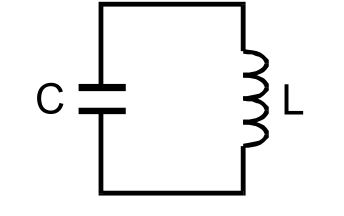
\includegraphics[height=3cm]{content/data/lckreis.jpg}
        \caption{Ungedämpfter Schwingkreis}
        \label{fig:lckreis}
    \end{subfigure}
    \begin{subfigure}{0.48\textwidth}
        \centering
        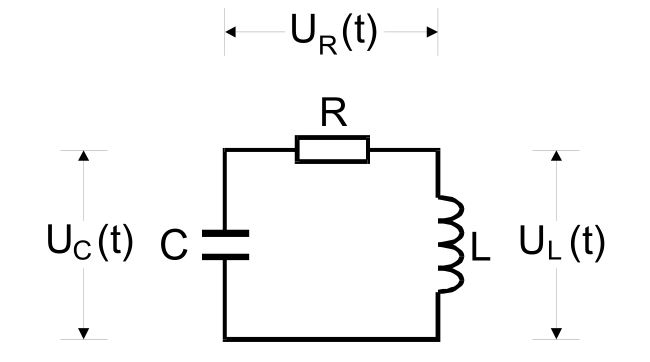
\includegraphics[height=3cm]{content/data/lrckreis.jpg}
        \caption{Gedämpfter Schwingkreis} 
        \label{fig:lrckreis}
    \end{subfigure}
    \caption{Schwingkreise mit den Bauelelementen: Kondensator mit Kapazität $C$, Spule mit Induktivität $L$, ohmscher Widerstand $R$.}
\end{figure}

\subsection{Differentialgleichungen und Lösungen zu den Schwingkreisen}
Nach dem 2. kirchhoffschen Gesetz, Induktionsgesetz und weiteren Beziehungen für die Spannung $U$, folgt für den LC-Kreis \ref{sec:lckreis} die Differentialgleichung
\begin{equation}
    \frac{\symup{d}^2I}{\symup{d}t^2} + \frac{R}{L} \frac{\symup{d}I}{\symup{d}t} + \frac{1}{LC} I = 0 .
    \label{eqn:dgl_lc}
\end{equation}
Der Ansatz
\begin{equation*}
    I(t) = \tilde{I} \mathrm{e}^{i\tilde{\omega} t} , \tilde{\omega}, \tilde{I} \in \mathbb{C}
\end{equation*}
löst die Differentialgleichung \autoref{eqn:dgl_lc}.
Es folgt
\begin{equation}
    \tilde{\omega}_{1,2} = i \frac{R}{2L} \pm \sqrt{\frac{1}{LC} - \frac{R^2}{4L^2}}
\end{equation}